%-------------------------------------------------------------------------
\ssect{Beam Elements}
\label{Section42}
%-------------------------------------------------------------------------

In this chapter we consider the finite element formulation 
for beams under bending conditions. 
Here, the theory according to Euler-Bernoulli is treated.

\sssect{Beam Theory according to Euler-Bernoulli for simple bending}

In this section we consider the Euler-Bernoulli beam element 
under pure bending conditions, i.e. without axial forces. 

{\bf Continuous Formulation:}
The equilibrium conditions can be derived from the 
infinitesimal beam element with the length $dx$. 
For the axial force $N(x)$, shear force $Q(x)$ and the 
moment $M(x)$, the following known differential equations 
are given

\begin{equation}
\renewcommand{\arraystretch}{1.5}
\left.
\begin{array}{rcl}
N(x) & := & 0 \\
\dfrac{d Q(x)}{dx} & = & - p(x) \\
Q(x) & = & \dfrac{d M(x)}{dx}
\end{array}
\right\}
\label{eq:balk1}
\end{equation}

with the loading function $p(x)$. Inserting equation
$(\ref{eq:balk1})_3$ in $(\ref{eq:balk1})_2$ yields the linear,
inhomogeneous, common differential equation of second order

\begin{equation}
\dfrac{d^2 M(x)}{dx^2} = - p(x) \; .
\end{equation}

\begin{Figure}[htb]
\begin{center}
\input{\dir/figbiege1.pstex_t}
\setlength{\baselineskip}{11pt}
\caption{Beam according to Euler-Bernoulli theory}
\label{figbiege1}
\end{center}
\end{Figure}%

The essential kinematic assumptions of the Euler-Bernoulli 
beam theory are 

\begin{enumerate}
\item constant cross-section and
\item "normal remains normal"
\end{enumerate}

The axial displacements in direction of the beam axis over 
the cross-section result from the assumption of constant 
cross-sections in

\begin{equation}
u(x,z) = z \cdot \beta(x) \, .
\end{equation}

For the definition of geometric quantities associated to 
the beam theory considered here, see Figure \ref{figbiege1}. 
The second Bernoulli-hypothesis yields

\begin{equation}
- \beta(x) = w'(x) \, ,
\end{equation}

with the deflections $w$. 
Hence, the strains in beam axis can be computed from the 
derivatives of the elastic line 

\begin{equation}
\ve_x = u,_x = z \cdot \beta' = - z \cdot w,_{xx}
\end{equation}

and in simplified notation we write 

\begin{equation}
\ve_x = - z w''(x) \, .
\label{eq:epsilonx}
\end{equation}

At first, we only analyze pure bending problems, i.e. 
no influence of axial force loads in beam axis are considered. 
The integral over the cross-section yields the bending moment 

\begin{equation}
M_y (x) = \int_{A} \sigma_x (x,z) \cdot z \, dA \, ,
\label{eq:momenty}
\end{equation}

wherein the normal stresses are calculated by Hooke's law

\begin{equation}
\sigma_x = E \cdot \ve_x \, .
\end{equation}

With equation (\ref{eq:epsilonx}) and (\ref{eq:momenty}) 
it follows

\begin{equation}
M_y (x) = \int_A - E z^2 w''(x) d A = - E w''(x) \int_A z^2 dA = -EI
w''(x) \, .
\label{eq:myw''}
\end{equation}

We obtain the shear force from the equilibrium equation 
(\ref{eq:balk1})${}_2$.
According to Bernoulli, the associated potential for a 
beam of length $l$ is

\begin{equation}
\Pi = \frac{1}{2} \int_l EI (w'')^2 dx - \int_l p\; w \; \, .
\label{eq:piw''q}
\end{equation}

{\bf Ansatz equations:}
We consider a typical element $k$ with the node numbers 
$i$ and $j$ for the FE-discretization, 
see Figure \ref{fig304}.
 
\begin{Figure}[htb]
\begin{center}
\input{\dir/fig3_04.pstex_t}
\setlength{\baselineskip}{11pt}
\caption{Definition of the beam element.}
\label{fig304}
\end{center}
\end{Figure}%

The second derivatives of the deflection $w$ appear in 
equation (\ref{eq:piw''q}), i.e. the constitutive 
equation have to be at least two-times continuously 
differentiable. We choose

\begin{equation}
\fbox{$\tilde{w}(\tilde{x}) = C_0 + C_1 \tilde{x} + C_2 \tilde{x}^2 +
C_3 \tilde{x}^3 $}\, .
\label{eq:ansatz}
\end{equation}

This assumption is

\begin{enumerate}
\item linearly independent (because we consider powers of $\tilde{x}$)
\item two-times continuously differentiable
\item geometrically conform (the completion of the boundary conditions, $w$ und $w'$, is possible). Geometrically conform
means, that the deflection and curvature at the boundary to 
the neighbour elements are continuous. 
The order of the differential equation in (\ref{eq:myw''}) 
is $2 n = 4$, i.e. $n=2$. 
The order of the derivatives of the essential boundary- and 
transition conditions is  $n-1=1$ with the Ritz method. 
\item sufficient for the description of, at least constant, 
internal force variables \\($M = -EI w''$ requires only 
quadratic ansatzfunctions for $w$ for this purpose)
\item sufficient for the description of rigid body deflections \\
(translation with $\tilde{w}= c_0$ and rotation with $\tilde{w} = C_0 + C_1\tilde{x}$).
\end{enumerate}

The computation of the derivatives of $\tilde{w}$ yields

\begin{equation}
\left.
\begin{array}{rcl}
\tilde{w}' (\tilde{x})  & = & C_1 + 2 C_2 \tilde{x} + 3 C_3 \tilde{x^2} \\
\tilde{w}'' (\tilde{x}) & = & 2 C_2 + 6 C_3  \tilde{x} \\
\tilde{w}''' (\tilde{x})& = & 6 C_3 \\
\tilde{w}'''' (\tilde{x})& = & 0
\end{array}
\right\} \, . 
\label{eq:ableitw}
\end{equation}

Due to the fact that the dependence $Q(x) \sim w'''(x)$ 
exists, we find that due to equation (\ref{eq:ableitw})${}_3$ 
the ansatz delivers the exact solution if we do not apply 
uniform loads. 
This coherence is also justifiable as follows: 
Because the ansatz (\ref{eq:ansatz}) satisfies the 
homogeneous differential equation $w''''= 0$, 
it describes a solution of equilibrium equation and 
delivers the exact solution in this case. 

\begin{Figure}[htb]
\begin{center}
\input{\dir/fig3_05.pstex_t}
\setlength{\baselineskip}{11pt}
\caption{Implementation of natural coordinates.}
\label{fig305}
\end{center}
\end{Figure}%

We use Hermite polynomials in the dimensionless quantity 
$\xi$ as ansatz function. 
The ansatz appears in the form

\begin{eqnarray*}
w(\xi) = N_1(\xi) w_1 + \bar{N}_1(\xi) \varphi_1 + N_2(\xi) w_2 +
\bar{N}_2(\xi) \varphi_2 = \bN^e \bd^e
\end{eqnarray*}

and has to satisfy the boundary conditions 

\begin{equation}
\left.
\begin{array}{rclccrcl}
w(\xi = -1) & = & w_1  & & w,_x (\xi = -1) & = & \varphi_1 \\
w(\xi = 1) &  = & w_2  & & w,_x (\xi = 1)  & = & \varphi_2 \\
\end{array}
\right\} \, .
\end{equation}

Herefrom we obtain 

\begin{equation}
\left.
\begin{array}{rclcrcl}
N_1 & = & \dfrac{1}{4}(2 - 3 \xi + \xi^3) &, &
N_2 & = & \dfrac{1}{4}(2 + 3 \xi - \xi^3) \\ [1.2ex]
\bar{N}_1 & = & \dfrac{1}{4}(1 - \xi - \xi^2 + \xi^3)\dfrac{l^e}{2} &, &
\bar{N}_2 & = & \dfrac{1}{4}(-1 - \xi + \xi^2 + \xi^3)\dfrac{l^e}{2} 
\end{array}
\right\} \;.
\end{equation}

\begin{Figure}[htb]
\begin{center}
\unitlength1cm
\begin{picture}(14,8)
\put(1,0){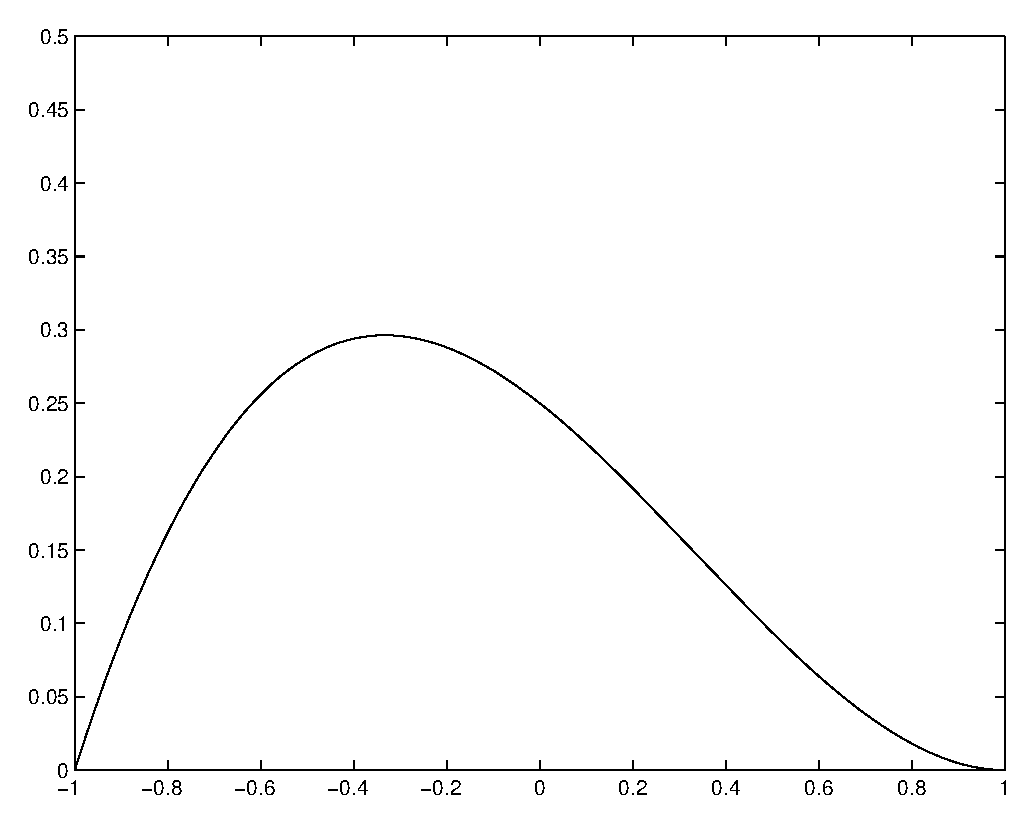
\includegraphics[width=.3\hsize]{\dir/herm3.eps}} 
\put(1,4){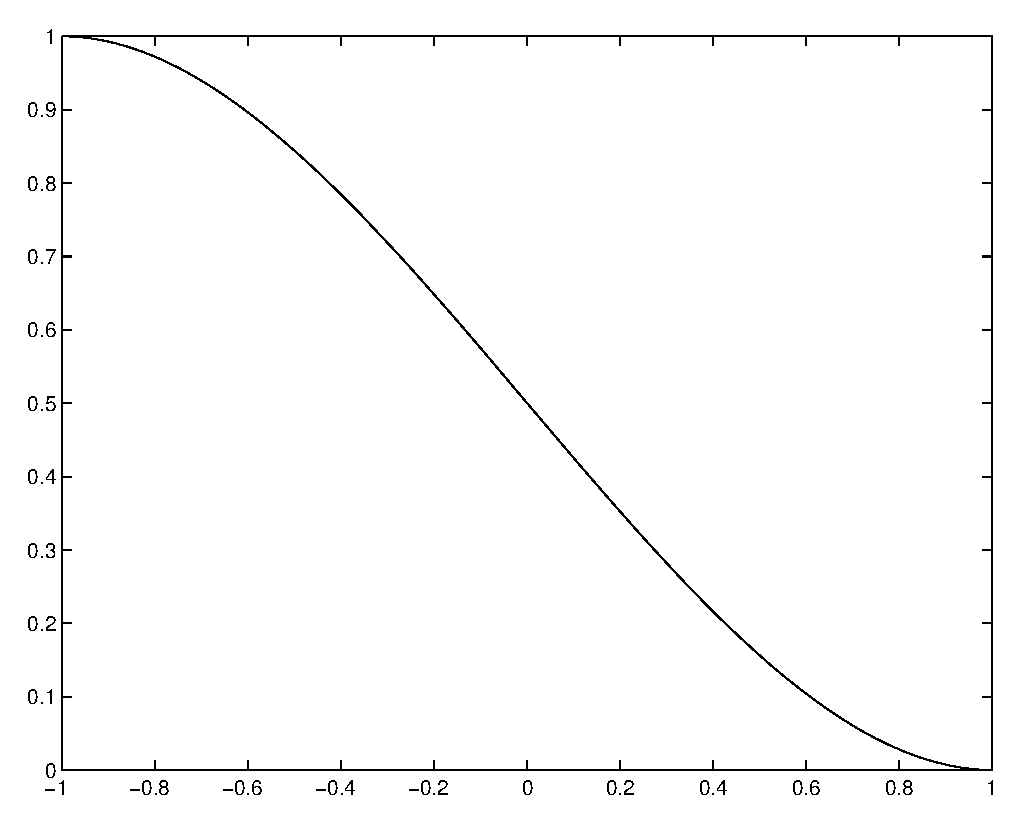
\includegraphics[width=.3\hsize]{\dir/herm1.eps}} 
\put(8,0){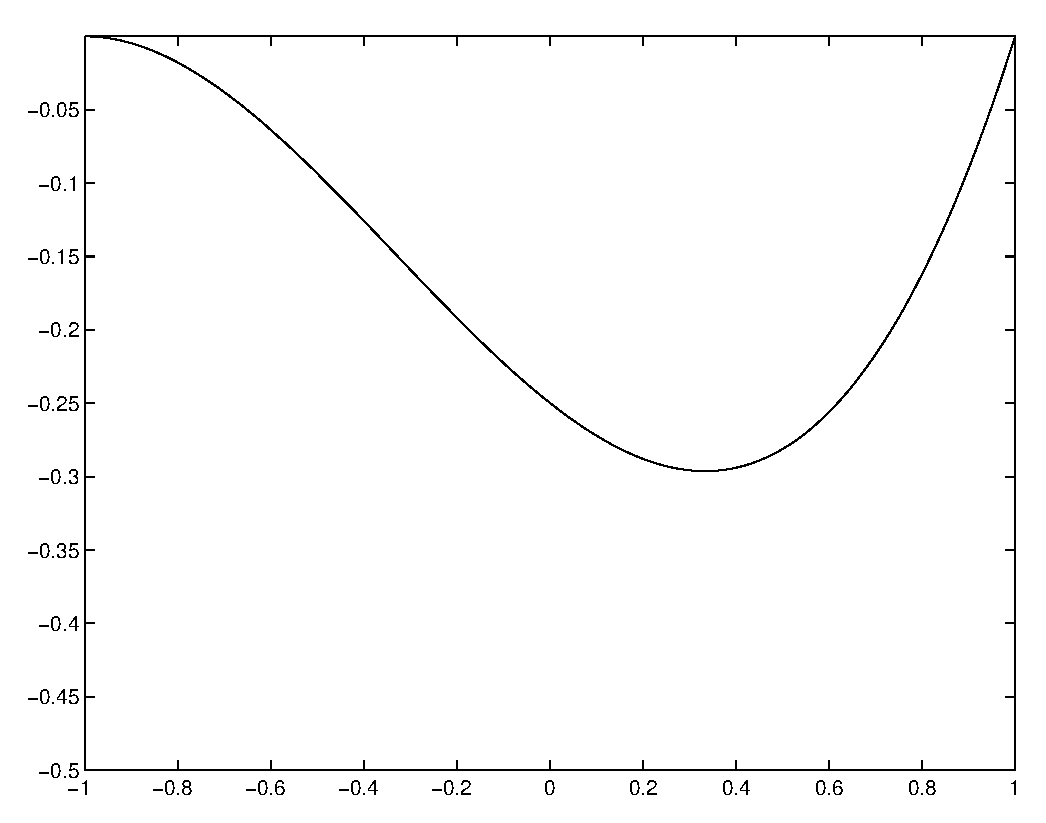
\includegraphics[width=.3\hsize]{\dir/herm4.eps}} 
\put(8,4){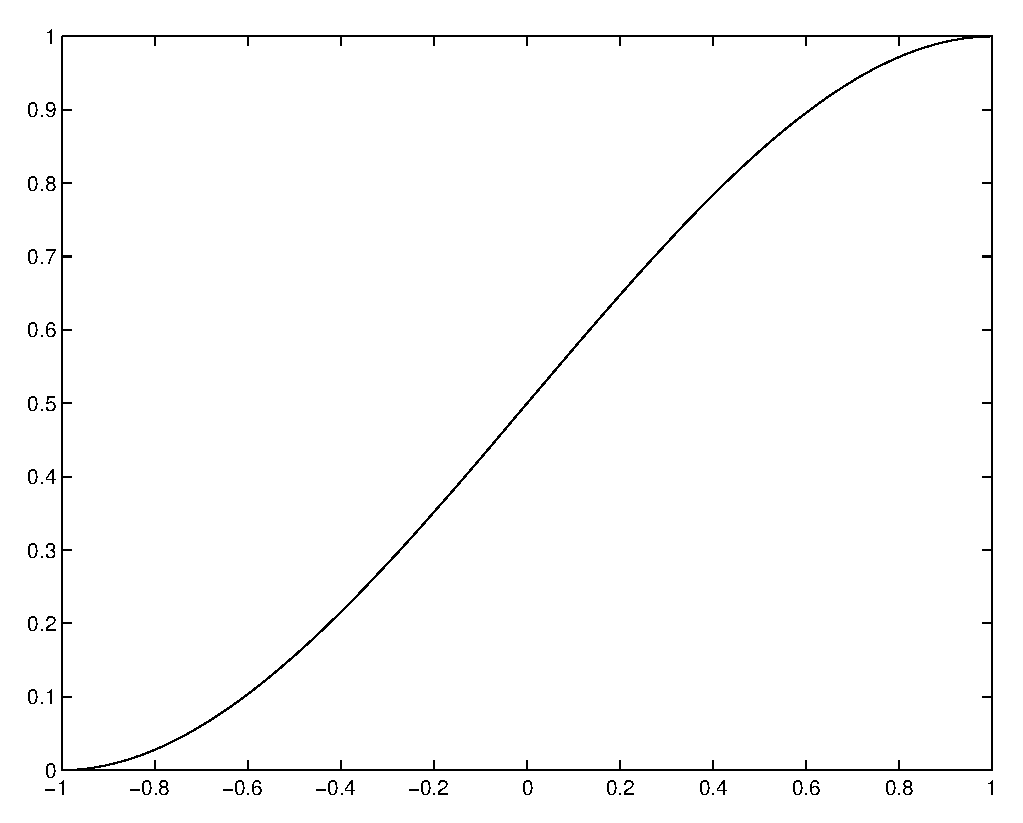
\includegraphics[width=.3\hsize]{\dir/herm2.eps}} 
\put(4,6){$N_1$}
\put(9,6){$N_2$}
\put(4,2){$\bar{N}_1$}
\put(9,2){$\bar{N}_2$}
\end{picture}
\caption{Hermite-polynomials}
\end{center}
\end{Figure}

By applying the chain rule

\begin{eqnarray*}
w' = \dfrac{dw}{dx} = \dfrac{dw}{d \xi} \dfrac{d \xi}{dx} = \dfrac{2}{l}
\dfrac{dw}{d \xi} 
\end{eqnarray*}

we receive

\begin{eqnarray*}
w' = N_{1, \xi} \dfrac{2}{l} w_1 + \bar{N}_{1, \xi} \dfrac{2}{l} 
\varphi_1 +
N_{2, \xi} \dfrac{2}{l} w_2 + \bar{N}_{2, \xi} \dfrac{2}{l} \varphi_2 \, .
\end{eqnarray*}

We obtain the second derivatives analogously with 

\begin{eqnarray*}
w'' = \dfrac{d^2w}{dx^2} = \dfrac{d^2w}{d \xi^2} \dfrac{d^2 \xi}{dx^2} 
= \dfrac{4}{l^2}
\dfrac{d^2w}{d \xi^2 } 
\end{eqnarray*}

to

\begin{equation}
w'' = \underbrace{\dfrac{4}{l^2}
\left[ 
\begin{array}{cccc}
N_{1, \xi \xi} & \bar{N}_{1, \xi \xi} & N_{2 , \xi \xi} & 
\bar{N}_{2, \xi \xi}  
\end{array}
\right]}_{\bB^e} \left[ 
\begin{array}{c}
w_1 \\ \varphi_1 \\ w_2 \\ \varphi_2
\end{array}
\right] = \bB^e \bd^e
\label{eq:bd}
\end{equation}

with the element displacement vector $\bd^{eT} = [ \begin{array}{cccc}
w_1 & \varphi_1 & w_2 & \varphi_2
\end{array}]$.

{\bf Discrete formulation:}
Starting from the minimum of the total potenial given in 
(\ref{eq:piw''q}) we obtain as a neccessary condition 

\begin{eqnarray*}
\delta \Pi = \int_l \delta w'' E I w'' d x - \int_l \delta w \;p \;dx = 0 \, 
\end{eqnarray*}

and the description for a typical element

\begin{eqnarray*}
\delta \Pi^{(e)} = \int_{l^e} \delta w''(x) E I w''(x) d x - 
\int_{l^e} \delta w(x)\; p(x) dx \; , 
\end{eqnarray*}

respectively. 
The transformation to the natural coordinates delivers 
with equation (\ref{eq:bd}) and \\ 
$\delta w'' = \bB^e \delta \,\bd^e$ and 
$dx = \dfrac{l}{2} d \xi$

\begin{eqnarray*}
\delta \Pi^{(e)} = \delta \bd^{eT} \int_{-1}^{1} \bB^{eT} EI \bB^e \,\dfrac{l}{2}\,
d\xi \, \bd^e - \delta \bd^{eT} \int_{-1}^{1} \bN^{eT} p \,\dfrac{l}{2}\, d\xi \, .
\end{eqnarray*}

Herefrom, we identify the element stiffness matrix $\bk^e$ 
and the element loading vector $\bp^e$ 

\begin{eqnarray*}
\bk^e := \int_{-1}^{1} \bB^{eT} EI \bB^e \,\dfrac{l}{2}\,
d \xi \qquad \and \qquad 
\bp^e = \int_{-1}^{1} \bN^{eT} p \,\dfrac{l}{2}\, d \xi \, .
\end{eqnarray*}

From this it follows, that

\begin{eqnarray*}
\bk^e = \dfrac{EI}{l^3} \left[
\begin{array}{cccc}
 12 &    6 l &  -12 & 6 l \\
6 l &  4 l^2 & -6 l & 4 l^2 \\
-12 & -6 l &   12 & -6 l \\
6 l &  4 l^2 & -6 l & 4 l^2
\end{array}
\right]
\end{eqnarray*}

and for $p(\xi) = \mbox{constant}$, we obtain

\begin{eqnarray*}
\bp^e = \dfrac{pl}{2} \left[
\begin{array}{c}
1 \\ l/6 \\ 1 \\ -l/6
\end{array}
\right] \; .
\end{eqnarray*}

The discrete total problem arises from

\begin{eqnarray*}
\delta \Pi = \sum_e \{ \delta \bd^{eT} \bk^{(e)} \bd^e - 
\delta \bd^{eT} \bp^{e} \} = 0 
\qquad \forall \quad \delta \bd^e
\end{eqnarray*}

and for the global problem we obtain 

\begin{eqnarray*}
\bK \bD = \bP \quad \with \quad 
\bK = \displaystyle \Assem \bk^{e} 
\end{eqnarray*}

whereby $\bK$ is the global stiffness matrix, 
$\bP$ the global loading vector and $\bD$ the global 
displacement vector. 

{\bf Calculation of the internal force variables: }
We compute the moment $M$ from the constitutive law 

\eb
M(\xi) = - EI w(\xi)_{,xx} = - EI \bB(\xi) \bd^e
\ee

Please note, that the location of evaluation has to 
be taken into account. 
For the definition of the internal force variables 

\eb
Q_l = - R_i \, , \quad M_l = M_i \, , \quad Q_r = R_j \, ,
\quad M_r = - M_j 
\ee

compare Figure \ref{definition_int_force_var}. 

\begin{Figure}[htb]
\begin{center}
\input{\dir/fig5_10.pstex_t}
\setlength{\baselineskip}{11pt}
\caption{Definition of the internal force variables with respect to a)
Finite-element-method and b) Statics.} 
\label{definition_int_force_var}
\end{center}
\end{Figure}%

The internal force variables are given by 

\eb
\renewcommand{\arraystretch}{2.0}
\left.
\begin{array}{l@{\, = \,}l@{\, = \,}l}
M_i & M(\xi = -1) & - \dfrac{EI}{l^2} [-6 , -4l , 6 , -2l] \bd^e \\
M_j & M(\xi = 1) & - \dfrac{EI}{l^2} [6 , 2l , -6 , 4l] \bd^e
\end{array}
\right\} \, , 
\ee

\newpage
whereas the shear force is not given by a constitutive law 
but computed via equilibrium

\eb
Q = M' = - \dfrac{EI}{l^2} \dfrac{2}{l} [6 , 3l , -6 , 3l] \bd^e
\, . 
\ee

{\bf Complete beam element}

Here we consider a complete beam element formulation, where 
also axial loads are taken into account, cf. Fig. \ref{fig5_11}. 

\begin{Figure}[ht]
\begin{center}
\input{\dir/fig5_11.pstex_t}
\setlength{\baselineskip}{1pt}
\caption{Completed flat beam element.}
\label{fig5_11}
\end{center}
\end{Figure}%

The flat Bernoulli beam with axial load and constant uniform load in $x-$ and $z-$ direction delivers 

\eb
\left[
\begin{array}{c}
R_{ix} \\ R_{iz} \\ M_i \\ R_{jx} \\ R_{jz} \\ M_j
\end{array}
\right]_L = \dfrac{E}{l} 
\left[
\begin{array}{cccccc}
A & 0 & 0 & -A & 0 & 0 \\
0 & 12 \dfrac{I}{l^2} & 6 \dfrac{I}{l} & 0 & -12 \dfrac{I}{l^2} &
6 \dfrac{I}{l} \\ 
0 & 6 \dfrac{I}{l} & 4I & 0 & -6 \dfrac{I}{l} & 4I \\
-A & 0 & 0 & A & 0 & 0 \\
0 & -12 \dfrac{I}{l^2} & -6 \dfrac{I}{l} & 0 &  12 \dfrac{I}{l^2} &
-6 \dfrac{I}{l} \\
0 & 6 \dfrac{I}{l} & 4I & 0 & -6 \dfrac{I}{l} & 4I
\end{array}
\right]_L
\left[
\begin{array}{c}
u_i \\ w_i \\ \varphi_i \\ u_j \\ w_j \\ \varphi_j
\end{array}
\right]_L - \dfrac{l}{2}
\left[
\begin{array}{c}
q_x \\ q_z \\ q_z \dfrac{l}{6} \\ q_x \\ q_z \\ -q_z \dfrac{l}{6}
\end{array}
\right]_L
\ee
\eb
\br_L^e = \bk_L^e \bd_L^e - \bp_L^e
\ee

in matrix notation. 
Since the above presented relations are applied to the 
description in the local coordinate system, a description 
with respect to a global coordinate system is neccessary for 
general boundary value problems.

$\rightarrow$ Transformation of the element relations is 
neccessary, cf. Figure \ref{transformation}

\begin{Figure}[htb]
\begin{center}
\input{\dir/fig5_12.pstex_t}
\setlength{\baselineskip}{11pt}
\caption{Transformation of coordinates} 
\label{transformation}
\end{center}
\end{Figure}%

\eb
\left[ \begin{array}{c} x_L \\ z_L \end{array} \right] =
\left[ \begin{array}{cc}
\cos \alpha & \sin \alpha \\
-\sin \alpha & \cos \alpha
\end{array} \right]
\left[ \begin{array}{c} x_G \\ z_G \end{array} \right]
\ee

The transformation for $u$, $w$ and $R_x$, $R_z$ respectively 
follows analogously, thus, we obtain 

\eb
\left[
\begin{array}{c}
u_i \\ w_i \\ \varphi_i \\ u_j \\ w_j \\ \varphi_j
\end{array}
\right]_L = 
\left[
\begin{array}{cccccc}
c & s & 0 & 0 & 0 & 0 \\
-s & c & 0 & 0 & 0 & 0 \\
0 & 0 & 1 & 0 & 0 & 0 \\
0 & 0 & 0 & c & s & 0 \\
0 & 0 & 0 & -s & c & 0 \\
0 & 0 & 0 & 0 & 0 & 1
\end{array}
\right]
\left[
\begin{array}{c}
u_i \\ w_i \\ \varphi_i \\ u_j \\ w_j \\ \varphi_j
\end{array}
\right]_G
\ee

with the abbreviation 

\begin{eqnarray*} 
c := \cos \alpha \\ s := \sin \alpha \, ,
\end{eqnarray*}

which can be reformulated by 

\eb
\bd_L^e = \bT^e \bd_G^e \, . 
\ee

The global stiffness matrix results from the discrete 
potential $\Pi^i=\sum_e \Pi^e$ 

\eb
\begin{array}{ll}
\Pi^i & = \dfrac{1}{2} \Assem \bd_L^{eT} \bk_L^e \bd_L^e
\\ & = \dfrac{1}{2} \Assem \bd_G^{eT} \bT^{eT} \bk_L^e
\bT^e \bd_G^e \\
 & =: \dfrac{1}{2} \Assem \bd_G^{eT} \bk_G^e \bd_G^e
\end{array}
\ee

to

\eb
\bK = \Assem \bk_G^e = \Assem \bT^{eT}
\bk_L^e \bT^e
\ee

global loading vector:

\eb
\bP = \Assem \bp_G^e = \Assem \bT^{eT}
\bp_L^e
\ee

\newpage
{\bf Example: }

\begin{Figure}[htb]
\begin{center}
\input{\dir/fig5_13.pstex_t}
\setlength{\baselineskip}{11pt}
\caption{Cantilever with loading case 1. (LC1) and loading case 2. (LC2)} 
\end{center}
\end{Figure}

FEM-calculation with one element

\begin{eqnarray}
\bK \bd = \bP
\end{eqnarray}

\begin{eqnarray}
\dfrac{EI}{l^3}
\left[ 
\begin{array}{cccc}
12 & 6l          & -12 &   6l \\
   & 4l^2        & -6l & 2l^2 \\
   & \mbox{sym.} &  12 &  -6l \\
   &             &     & 4l^2 \\
\end{array} 
\right]
\left[ 
\begin{array}{c}
w_1 \\ \varphi_1 \\ w_2 \\ \varphi_2
\end{array} 
\right] = &
\underbrace{
\left[ 
\begin{array}{c}
1 \\ \frac{l}{6} \\ 1 \\ - \frac{l}{6}
\end{array} 
\right] q \dfrac{l}{2}}_{\Disp LC1}  
\;\; \mbox{and} \, =& 
\underbrace{
\left[ 
\begin{array}{c}
0 \\ 0 \\ F \\ 0
\end{array} 
\right]}_{\Disp LC2} \, . 
\end{eqnarray}

We implement the boundary conditions 

\begin{eqnarray}
w(0) = 0 & \rightarrow & w_1 = 0 \\
w'(0) = \varphi(0) = 0 & \rightarrow & \varphi_1 = 0
\end{eqnarray}

and eliminate the first and second row/ column and 
obtain 

\begin{eqnarray}
\dfrac{EI}{l^3} \left[ \begin{array}{cc}
12 & -6l \\ -6l & 4l^2 \end{array} \right]
\left[ \begin{array}{c} w_2 \\ \varphi_2 \end{array} \right] = & 
\underbrace{
\left[ \begin{array}{c} q \frac{l}{2} \\ -q \frac{l^2}{12} \end{array}
\right]}_{\Disp LC1}
\quad \mbox{and} \quad =& 
\underbrace{
\left[ \begin{array}{c} F \\ 0 \end{array} \right]
}_{\Disp LC2} \mbox{respectively.} 
\end{eqnarray}

The reduction of the system of equations delivers

\begin{eqnarray}
\varphi_2 = \dfrac{ql^3}{6EI} \, , & w_2 = \dfrac{ql^4}{8EI} & \quad
\mbox{LC1} \\ 
\varphi_2 = \dfrac{Fl^3}{2EI} \, , & w_2 = \dfrac{Fl^3}{3EI} & \quad
\mbox{LC2}
\end{eqnarray}
{\bf Note with respect to loading case 1:} \\
Exact solution $\rightarrow$ cubical $w$ \\
FE-ansatz for $w$ is cubic \\
$\rightarrow$ exact elastic curve and exact internal force variables

{\bf Note with respect to loading case 2:} \\
Exact solution $\rightarrow$ quadratic $w$ \\
FE-ansatz for $w$ is cubic \\
$\rightarrow$ not exact, but the kinematic quantities 
at the nodes are exact


\newpage
{\small
\begin{verbatim}
      subroutine
 elmt06(d,ul,xl,ix,tl,s,p,ndf,ndm,nst,isw)
c-----------------------------------------------------------------------
c     elmt06  : Two-dimensional beam element
c
c     List of parameters
c       d(1-2)       material- and element parameters
c       d(1) = yo    - modulus of elasticity
c       d(2) = moin  - geometrical moment of inertia
c       ul(ndf,*)    solution vector
c       xl(ndm,nel)  joint coordinates
c       s(nst,nst)   stiffness matrix
c       p(nst)       residual
c       ndf          number of degrees of freedom 
c       ndm          dimensions of the joints
c       nst          number of degrees of freedom of the elements
c       isw          execution parameters
c-----------------------------------------------------------------------
      implicit none
      include   'bdata.h'
      include   'cdata.h'
      include   'debugs.h'
      include   'eldata.h'
      include   'iofile.h'
      integer ix(*)
      integer ndf,ndm,nst,isw
      integer ll,i,j,l
      real*8 d(*),ul(ndf,*),xl(ndm,*),tl(*),s(nst,nst),p(*)
      real*8 bmat(nst),btc(nst)
      real*8 sg(2),wg(2)
      real*8 vl(4),momnod(2)
      real*8 yo,moin,sl,dvol,dy,wxx,mom
      logical errck,pinput
c
      if(isw.eq.1) then
c-----------------------------------------------------------------------
c...  Import of material values
    1 if(ior.lt.0) write(*,3000)
        errck=pinput(d,2)
	if(errck) go to 1
        if(ior.lt.0) then
	  write(*,2000) d(1),d(2)
	end if
	write(iow,2000) d(1),d(2)
c
      elseif(isw.eq.2) then
c-----------------------------------------------------------------------
c...  element check with respect to mistakes
        if(d(2) .le. 0.d0) then
          write(*,*)' geometrical moment of inertia .le. 0'
          stop
        endif
c
      elseif(isw.eq.3 .or. isw.eq.4) then
c-----------------------------------------------------------------------
c...  Calculation of the stiffness matrix and of the residual
c...  Material- and element parameters
        yo    = d(1)
        moin  = d(2)
c...  Length
        sl = xl(1,2) - xl(1,1)
	dy = xl(2,2) - xl(2,1)
	if (dy .gt. 1.e-9 .or. dy .lt. -1.e-9) then
	  write(*,*) 'Only horizontal beam elements'
	  write(*,*) 'are allowed in the basic version!'
          stop
	end if
c...  Calculation of the local displacements
	call pzero(vl,4*1)
        vl(1) = ul(1,1)
        vl(2) = ul(2,1)
        vl(3) = ul(1,2)
        vl(4) = ul(2,2)
c...  Number of Gauss-points and calculation of the nodes  
        ll = 2
        sg(1) = - 1.d0/dsqrt(3.d0)
        sg(2) = + 1.d0/dsqrt(3.d0)
        wg(1) = 1.d0 
        wg(2) = wg(1)
c.... Gauss loop
        do l = 1,ll
          dvol = 0.5d0*sl*wg(l)
          call pzero(bmat,nst)
          call bmat06(bmat,sg(l),sl)
c...  Calculation of w''(xi) 
	     wxx = 0.d0
	     do j=1,nst
              wxx = wxx + bmat(j)*vl(j)
	     end do
c...  Calculation of internal force variables (Moment) (at Gauss-points)
	  mom = yo*moin*wxx
          if(isw .eq. 4)then
c.... Output instructions, internal force variables (at joints) in the output file,
c                Usage of convention of internal force variables of the statics
         if (l.eq.1) then
	      momnod(1) = -1.d0*(yo*moin/(sl*sl))*(-6.d0*vl(1) -
     &                 4.d0*sl*vl(2) + 6.d0*vl(3) - 2.d0*sl*vl(4))
	      momnod(2) = -1.d0*(yo*moin/(sl*sl))*(6.d0*vl(1) +
     &                 2.d0*sl*vl(2) - 6.d0*vl(3) + 4.d0*sl*vl(4))
	      write(*,100)
	      write(*,101)
	      write(iow,100)
	      write(iow,101)
	    end if
            write(*,103) ix(l),xl(1,l),xl(2,1),momnod(l)
            write(iow,103) ix(l),xl(1,l),xl(2,1),momnod(l)
c
          elseif(isw .eq. 3)then
c...  Calculation of the residual
            do i=1,nst
	      p(i) = p(i) - bmat(i)*mom*dvol
	    end do
c...  Compute B^T C
	    call pzero(btc,4*1)
            do i  = 1,nst
              btc(i) = bmat(i)*yo*moin*dvol
            enddo
c...  Compute B^T C B = stiffness matrix
            do i  = 1,nst
              do j  = 1,nst
                s(i,j) = s(i,j) + btc(i)*bmat(j)
              enddo
            enddo
          endif    ! End of calculation of local stiffness matrix
        end do   ! Gauss-loop
c
c
      endif   !isw=1,2,3,4,5,6,7,8
c
c----------------------------------------------------------------------
c...  format instructions
 100  format(15x, 'internal force variables')
 101  format(4x,'joint',3x,'x',5x,'y',8x,'M')
 103  format(5x,i3,2x,f5.2,1x,f5.2,1x,e12.5)
2000  format(5x,'beam element:'//
     &   5x,'modulus of elasticity                   yo = ',e12.5/
     &   5x,'geometrical moment of inertia           moin = ',e12.5/)
3000  format(' Input: Yo,moin'/'   >',$)
      end
c
c
c
      subroutine bmat06(bmat,xi,sl)
c--------------------------------------------------------------------72
c     Calculation of the B-operator
c       List of parameters
c       bmat(4)  B-operator
c       xi         Gauss-point
c       sl         Length of element
c----------------------------------------------------------------------
      implicit none
      real*8 bmat(4)
      real*8 sl,xi
c
c...  Calculation of the B-operator
      bmat(1) = 6.d0*xi/(sl*sl)
      bmat(2) = -1.d0/sl + 3.d0*xi/sl
      bmat(3) = - 6.d0*xi/(sl*sl)
      bmat(4) = 1.d0/sl + 3.d0*xi/sl
      return
      end
c
\end{verbatim}
}

